\documentclass{FR16} 
\usepackage{listings}
\usepackage{pdfpages}
\usepackage{subfiles} 
\usepackage{graphicx}

\begin{document}

\maketitle

% ML template reports
% https://www.cs.utexas.edu/~mooney/cs391L/paper-template.html
%https://github.com/udacity/machine-learning/blob/master/projects/capstone/report-example-1.pdf
\newpage
\tableofcontents
\newpage
\listoffigures
\newpage
\section{Abstract}
The aim of the project is to analyse, develop prediction models and define  clusters of the data from "New York City Airbnb Open Data" Kaggle competition.
\\ One part of the study is focused on the development of predictive models to forecast house prices using these Supervised Learning technics:\begin{itemize}
\itemsep0em 
\item Linear Regression
\item Decision Tree
\item Random Forest
\item Ranger Random Forest
\item Neural Networks
\end{itemize}
For each of these, a comparison between the Mean Square Error of all methods has been made to highlight which have the best performance. Also, for training all models, multiple subsets of the dataset has been applied: filter by neighbourhood group and filter by neighbourhood group and room type. In this way, is possible to give an overview of the result for each case.\\\\
The second part is focused on the cluster and data reduction technics using these Unsupervised Learning technics:
\begin{itemize}
\itemsep0em
\item K-means Algorithm and Clustering for mixed-type data
\item Hierarchical clustering
\item Principal Component Analysis for mixed-type data
\end{itemize}

%%Eachreport must contain:\\
%•shortabstract: what are your going to present %in the report\\
%•statementof the problem/goalof the analysis %and description of thedata set(s)\\
%•list of three to fivefindings/keypoints\\
%•the analysis with wisecommentary\\
%•(optional) theoretical background of the used %methods\\
%•conclusions(should include the findings/%keypoints)\\
%•theAppendix, containing all the R codeNotice:
%\\•Thepaper lengthisirrelevant provided that %the content is correct.
%\\•No R code in the main text.The R code must %be confined to the appendix\\
%•The report should be prepared inPDFonly

\newpage
\section{Problem Definition and Algorithm}
\subsection{Two main Goals}

\subsubsection{Develop predictive models for price}
The first objective is the forecast of the prices. This could be useful for a lot of scenarios. For example, from a Airbnb customer point of view, he/she would like to get the list of houses more in line with his/her preference choice, or for a host point of view, where given the position and other information he/she could get a suggestion of the per day price of his property in New York City. 

\subsubsection{Define clusters and groups}
The second objective is the definition of group between the houses with different characteristics. For a user point of view could be useful to have information about available houses similar to those booked in the past. This could be also useful after the booking for a suggestion analysis having the information about last booked houses in New York or houses in similar cities around the world. Another important analysis, could be determine which are the most important features that describe better the data. 
\newpage
\subsection{Algorithms}
\subsubsection{Linear Regression}
 Linear regression  is a linear approach to modelling the relationship between a dependent variable and one or more independent variables. 
 
  \subsubsection{Decison Trees}
In decision analysis, a decision tree can be used to represent decisions visually and explicitly and decision making.


 \subsubsection{Random Forest}
 Random forests are an ensemble learning method for classification, regression, and other tasks that operate by constructing a multitude of decision trees.
 \subsubsection{Ranger Random Forest}
Ranger is a fast implementation of random forests or recursive partitioning, particularly suited for high dimensional data. 

\subsubsection{Neural Networks}
Neural networks are a set of algorithms, modelled  loosely after the human brain, that are designed to recognize patterns.

\subsubsection{K-means}
K-means is a method of vector quantization, originally from signal processing, that aims to partition n observations into k clusters in which each observation belongs to the cluster with the nearest mean.

\subsubsection{Principal Component Analysis}
PCA produces a low-dimensional representation of a
dataset. It finds a sequence of linear combinations of the
variables that have maximal variance, and are mutually
uncorrelated. Apart from producing derived variables for use in
supervised learning problems, PCA also serves as a tool for
data visualization.

\newpage
\section{Experimental Evaluation}

\subsection{Methodology}
\subsubsection{Data Inspection}
The dataset is part of a Kaggle competition, called the New York City Airbnb Open Data. It contains 48.000 rows per 16 columns.
The dataset is structured with these columns: 
\begin{itemize}
\itemsep0em 
\item \textbf{id}
\item \textbf{name}: name of the listing
\item \textbf{host\_id}
\item \textbf{host\_name}
\item \textbf{neighbourhood\_group}: location
\item \textbf{neighbourhood}: area
\item \textbf{latitude}: coordinates
\item \textbf{longitude}: coordinates
\item \textbf{room\_type}: space type
\item \textbf{price}:  in dollars
\item \textbf{minimum\_nights}: amount of nights minimum
\item \textbf{number\_of\_reviews}: number of reviews
\item \textbf{last\_review}: latest review
\item \textbf{reviews\_per\_month}: number of reviews per month
\item \textbf{calculated\_host\_listings\_count}: amount of listing per host
\item  \textbf{availability\_365}: number of days when listing is available for booking\\
\end{itemize}
It has been selected only 5 of these variables: price, latitude, longitude, neighbourhood\_group and room\_type. It is reasonable to select them to predict the prices and to obtain different clusters. The position and the neighbourhood are important since if a property is positioned near the city centre will have a higher price with respect to those situated in the outskirts; also the type of room, since an entire apartment will cost more than a single room. \\\\
From the Figure \ref{fig:1} is possible to see the distribution of the price. The minimum price is $0$ and the maximum is $10000\$$. Price has been filtered with a value greater than  $15\$$ since it is not possible to rent a house for free. Moreover, a luxury house cost a lot per day, but these values cannot be consider in the model, instead they are outliers and for this reason it is convenient to filter the price again and take those that have a value lower than $500\$$. The reason is that the third quantile has a price distribution of $175\$$ which is a far from $10000\$$ (Figure \ref{fig:3}). It has also been checked the null and missing value  in the dataset and has not been found apart from the reviews\_per\_month column. It is not a problem, since this last feature has been not taken in account to train the models. 
\\
\begin{figure}[H]
\centering
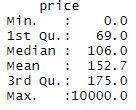
\includegraphics[width=0.3\textwidth]{figures/figure1.jpg} 
\caption{\label{fig:1}Price summary}
\end{figure}
\noindent From Figure \ref{fig:2}, it is possible to see the distribution of all houses in New York City and the price. This picture is not  informative since it can be noticed that the prices for the most part are in the range $0$-$500\$$ and only a low number of instances have a price greater than $500\$$. Deleting the outliers, the Figure \ref{fig:3} is more informative than the one before.

\begin{figure}[!htb]
   \begin{minipage}{0.48\textwidth}
     \centering
     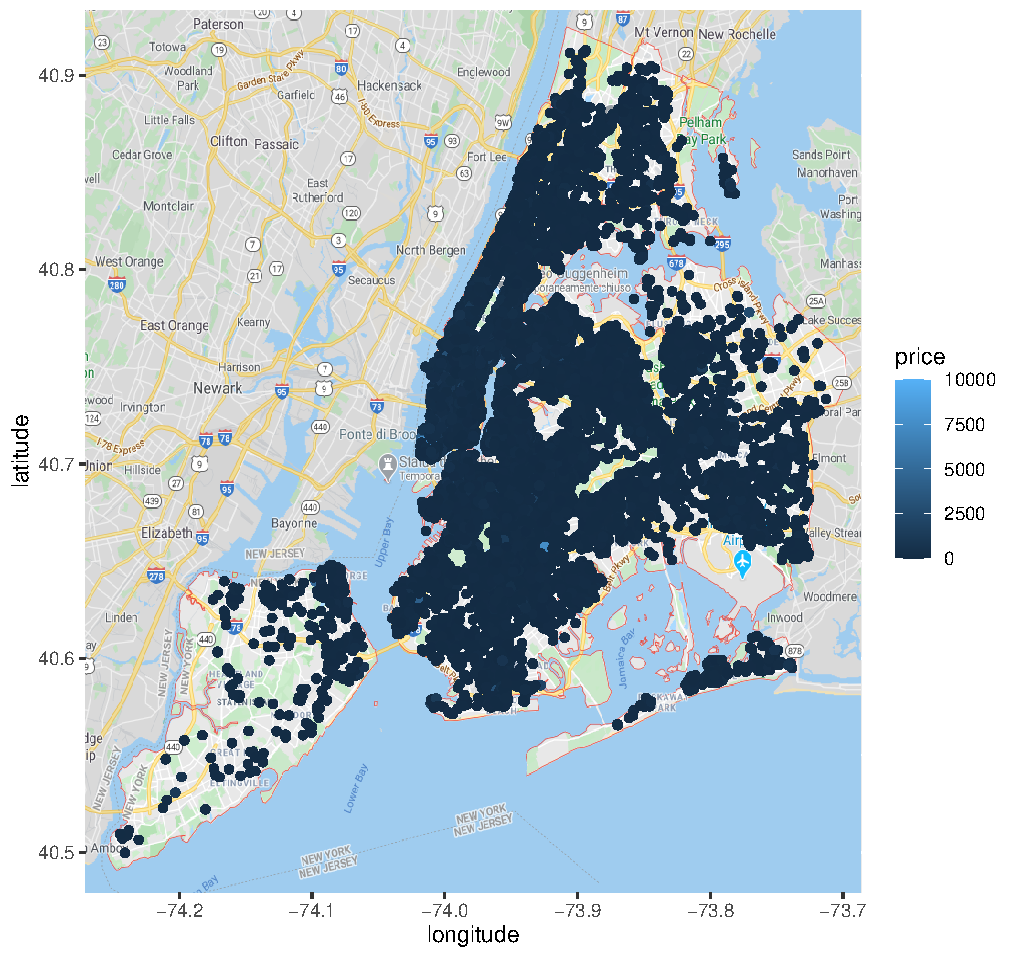
\includegraphics[width=1\linewidth]{figures/figure2.pdf} 
     \caption{\label{fig:2}Distribution of all houses in NY colored by prices}

   \end{minipage}\hfill
   \begin{minipage}{0.48\textwidth}
     \centering
     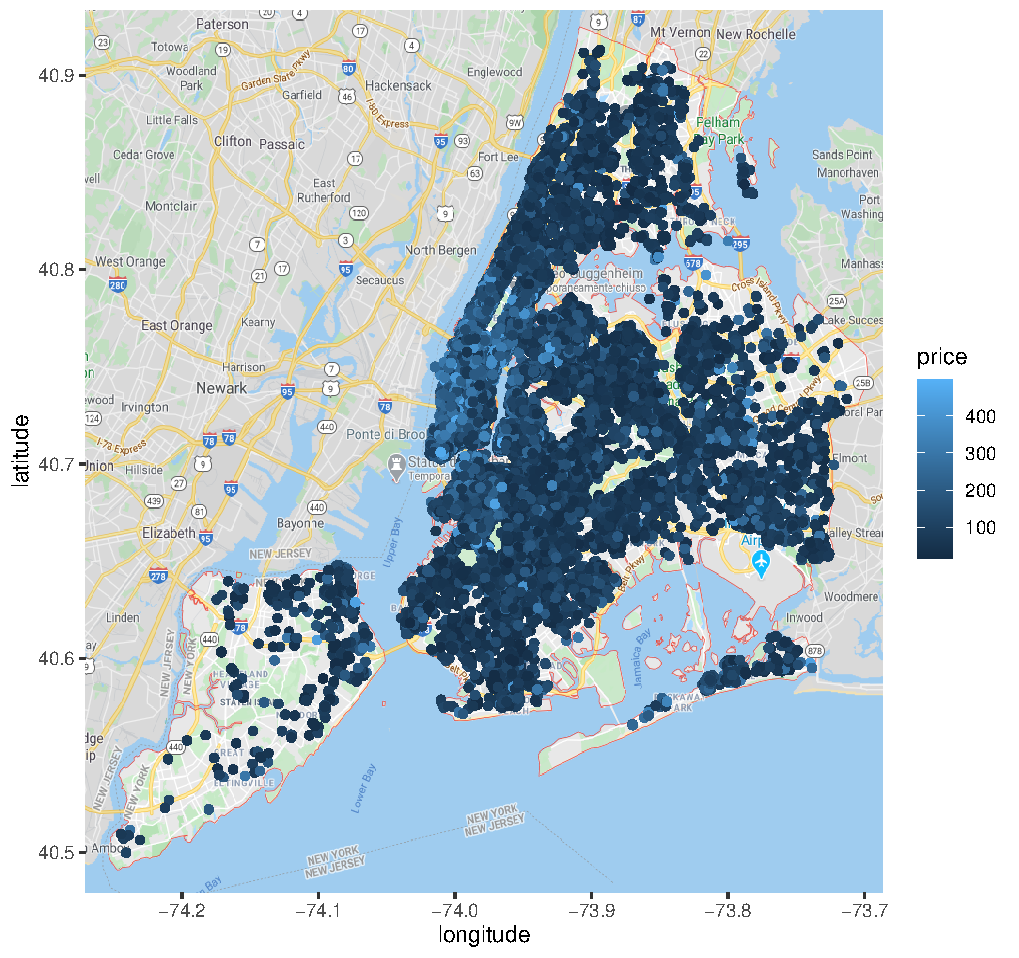
\includegraphics[width=1\linewidth]{figures/figure3.pdf}
     \caption{\label{fig:3} Distribution of all houses in NY of price between $15\$$ and $500\$$ per day}

   \end{minipage}

\end{figure}

\newpage
\subsubsection{Data Cleaning and Pre-processing}

The dataset has approximately 48.000 rows for each column and due to the large amount of data, an important part of the work is related to the pre-processing. Some variable has been rescaled to let the models to learn faster and better and to perform a better prediction. Latitude and longitude have not been rescaled for forecast price model, while have being rescaled in cluster analysis for a consistent distance calculation. Categorical variables have also been rescaled assigning a numerical value to each category, resulting as unordered factors.\\
The selected categorical variables are: neighbourhood\_group and room type.\\
The selected numerical variables are: latitude, longitude and price.
\\\\
Considering that every neighbourhood group and room type could impact the prices in different way for each singular case, different subsets (Figure \ref{fig:4}) of the original dataset have been define and to then try different methods of forecast. This is because a customer should choose which of the different neighbourhood and room type is interested in and not only been generalised to the all New York city houses. Models have been built for different scenarios : users interested in all New York City houses and all type of room, users interested only in a single neighbourhood and users interested in a single neighbourhood and a single room type. 
\\ Including all different scenarios could be computationally expensive for large dataset, but in this case the training proceeded without any problem. \footnote{ The models have been trained on a machine with quad-core 3.5 GHz processor, 8 Gb RAM and 4 Gb dedicated GPU.} Computational problem may emerge for the case of hyper parametrisation  tuning, even using multiprocessing and multithreading technics. For semplicity, in this project no model tuning has been made. \\
Also, for clustering have been filter every scenario, but not for the case of Hierarchical Clustering because otherwise it would generate a unreadable dendrogram. For this reason, it has been calculated the mean of all neighbourhood and room type price case. 


\begin{figure}[H]
\centering
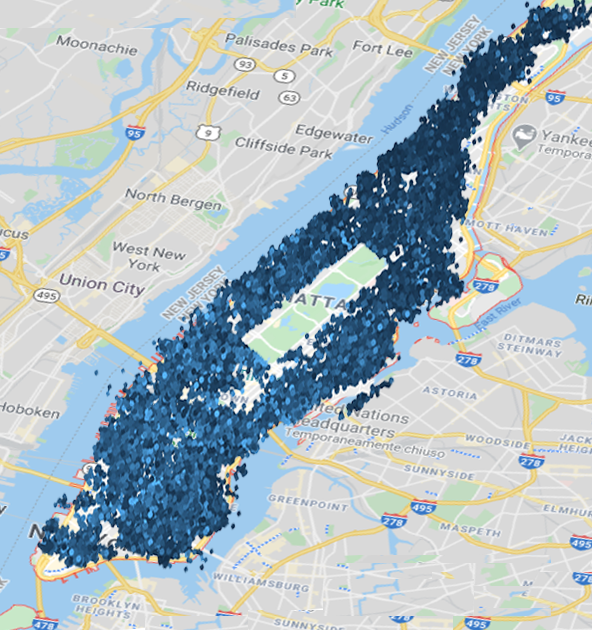
\includegraphics[width=0.5\textwidth]{figures/figure4.PNG} 
\caption{\label{fig:4}  Approximated distribution map of all houses in Manhattan }
\end{figure}






\newpage


\subsection{Results}

Since the number of models trained are very high, the study result will be presented for different macro groups that depend on the different subset of the dataset: entire dataset,  filtering by neighbourhood  and filtering by neighbourhood  and room type. This because neighborhood in general have similar result (like Manhattan has similar shape of Brooklyn and Staten Island has a similar shape of Bronx).\\\\


\subsubsection{Linear Regression Results}
%Linear Regression has been applied to the different subset and gains different results based on the macro group.

\textbf{Linear Regression on the entire dataset}\\
\noindent The results on the entire dataset are acceptable. All variables are significant for the model and the $R^2$ value is 40\% (Figure \ref{fig:6}).
The Mean Square Error (Figure \ref{fig:5}) has a value of 0.6 which is acceptable. All the neighbourhood groups have a positive effect on the price apart for the $4^th$ one. This could be because Staten Island does not have expensive houses compared to the other group. \\
Also, the latitude and longitude have a slight negative effect on the price. Entire apartment has a slight positive effect while the shared house negative. This could be because entire house will cost more than a shared room, so the price will increase for this type of room. 

\begin{figure}[H]
\centering
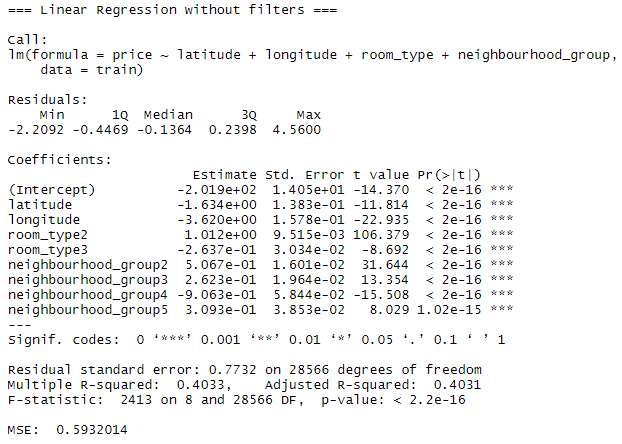
\includegraphics[width=0.5\textwidth]{figures/lm1.PNG} 
\caption{\label{fig:6} Linear Regression output for the entire dataset}
\end{figure}
\newpage
\noindent \textbf{Linear Regression for specific neighbourhood group}

\noindent Models give different results for the specific neighbourhood group. For the first three (Brooklyn, Manhattan and Queens) $R^2$ are over approximately $30\%$. For the MSE, the values have different ranges based on the distribution of prices in the singular neighbourhood. To be noticed, is the fact that MSE of Brooklyn is significantly lower with respect to Manhattan, given the have a similar number of houses and have almost the same price distribution. The only difference between the two is the fact that Manhattan has more entire apartment type of room. 
\\ All variables have a significant effect on the price apart for the latitude in Manhattan and longitude for Queens with a 0.1.  \\
For the last two groups (Staten Island and Bronx) all variables do not have significance in the response variable apart for the Entire Apartment dummy which have a positive effect. This is because entire properties will cost more than shared rooms.
\begin{figure}[H]
\centering
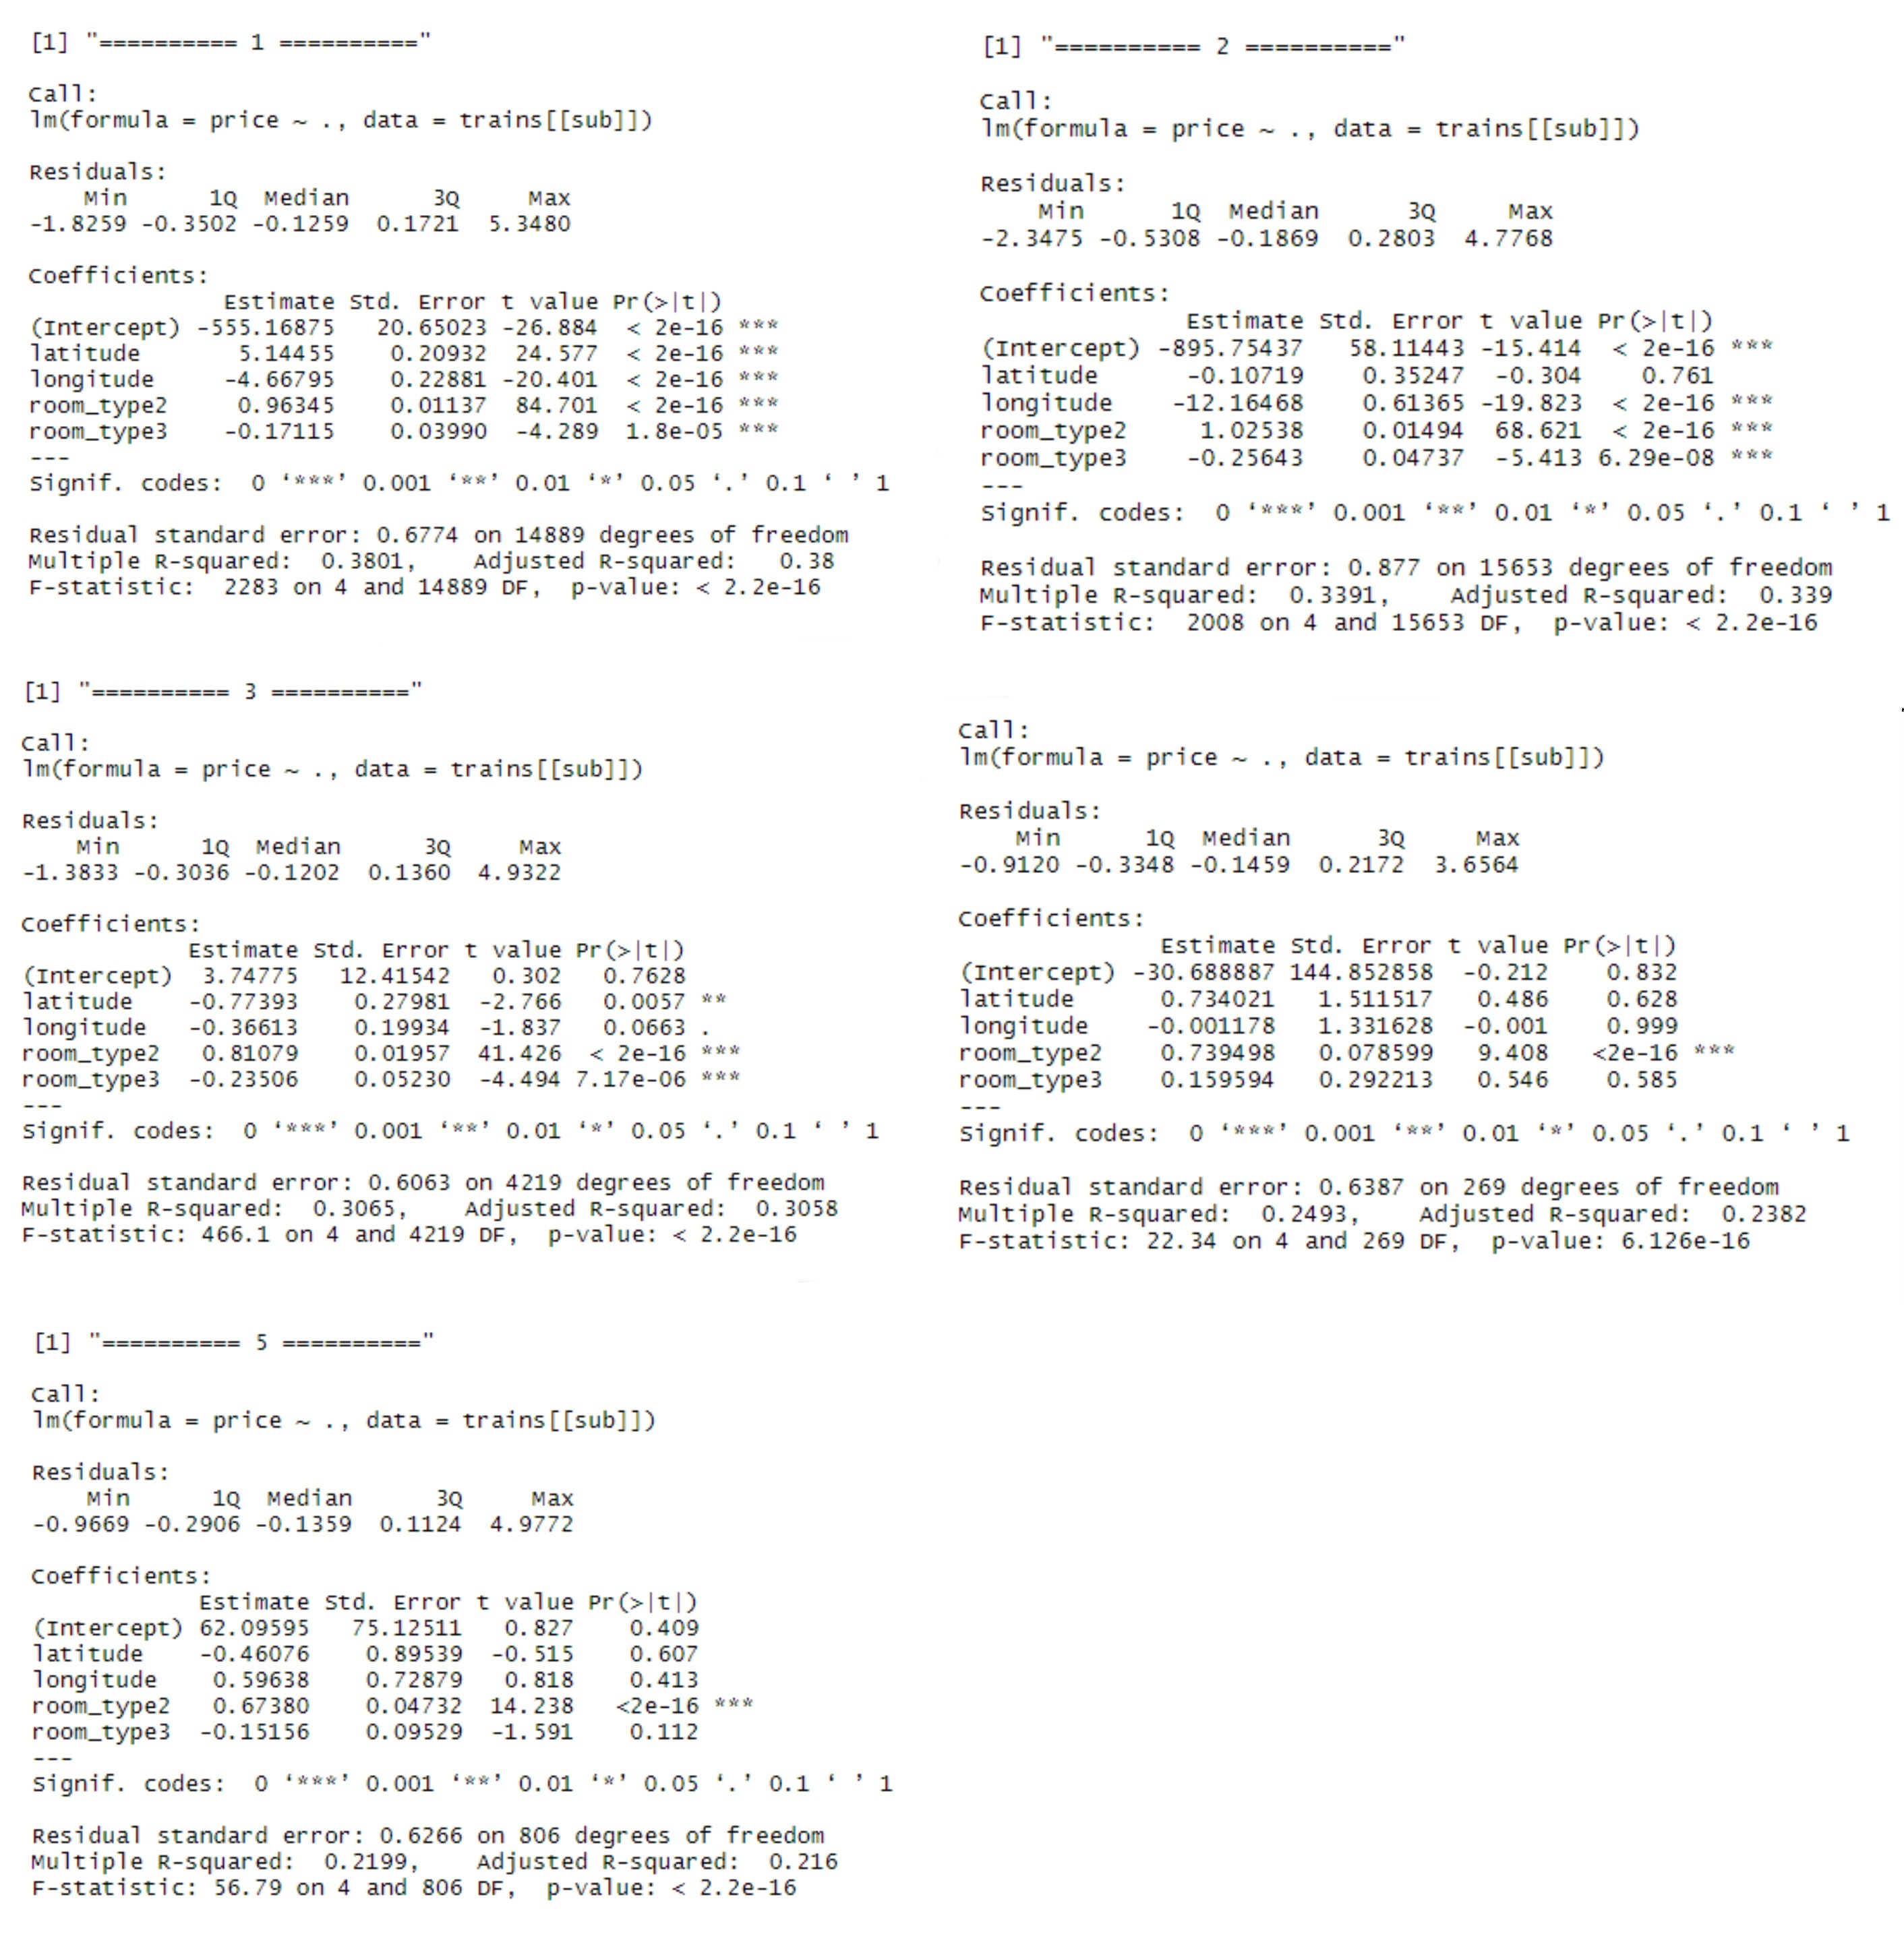
\includegraphics[width=0.8\textwidth]{figures/lm2.jpg} 
\caption{\label{fig:6}  Linear Regression output filtering by  Manhattan}
\end{figure}

\newpage
\noindent \textbf{Linear Regression for specific neighbourhood group and room type}\\
\noindent Adding a filter also for the room type, models give acceptable results in some cases and not in others. (Figure \ref{fig:7}) 
For the larger subset the model confirms the significant of the variables, apart for latitude in Manhattan such as happened in the model using this neighbourhood data. In Manhattan with Entire apartment model, instead, all variables have a significant effect. For the remaining neighbourhood groups the variables do not result as significant in the model. This could be because the subset obtained from this filtering are not large ( they have less than 300 rows). Also, in all model the $R^2$ result to be lower than $10\%$ but this depends on the fact to train they have less information.
\\
Also, in this model the MSE of Brooklyn is lower in all the type of room type than the Manhattan MSE. 
\begin{figure}[H]
\centering
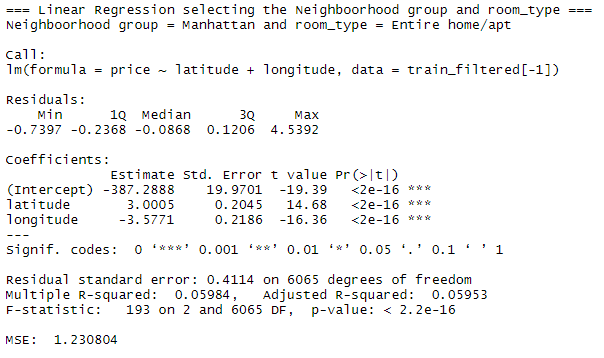
\includegraphics[width=1\textwidth]{figures/lm3.PNG} 
\caption{\label{fig:7}  Linear Regression output filtering by  Manhattan and Entire home/Apartment }
\end{figure}




\newpage 
\subsubsection{Decison Trees Results}
\textbf{Decison tree  without filters}\\
\noindent For the entire dataset, the MSE has a value of $0.605$ (Figure \ref{fig:9}) Important to be notice is the fact that the neighbourhood groups variable have not been used in the construction of the tree. Moreover, what really influence the price is the type of room (Figure \ref{fig:10}).


\begin{figure}[!htb]
   \begin{minipage}{0.48\textwidth}
     \centering
     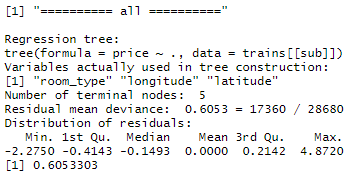
\includegraphics[width=.7\linewidth]{figures/dt.PNG} 
     \caption{Decision Tree results on the entire dataset}\label{fig:9}
   \end{minipage}\hfill
   \begin{minipage}{0.48\textwidth}
     \centering
     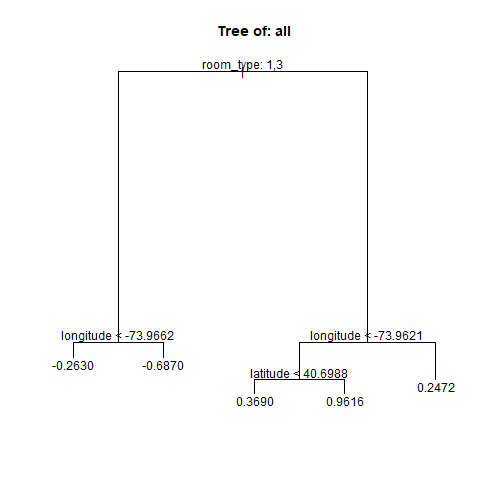
\includegraphics[width=.7\linewidth]{figures/tree-all.PNG}
     \caption{Tree generated for the entire dataset}\label{fig:10}
   \end{minipage}
\end{figure}


\noindent \\ \textbf{Decision tree for specific neighbourhood group}\\
\noindent For the specific neighbourhood group decision tree models give output similar MSE results with respect to the Linear Regression. Also, in this case, the latitude for Manhattan has not been used in the model to predict the price (Figure \ref{fig:11}). 

\begin{figure}[!htb]
   \begin{minipage}{0.48\textwidth}
     \centering
     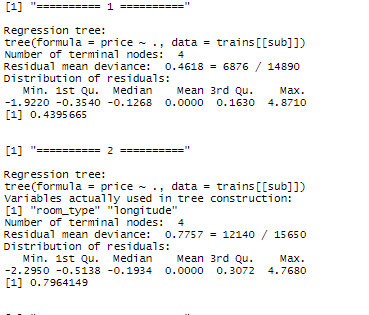
\includegraphics[width=.7\linewidth]{figures/dt1.1.PNG} 
   \end{minipage}\hfill
   \begin{minipage}{0.48\textwidth}
     \centering
     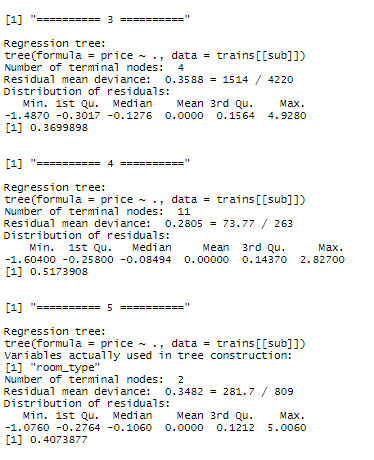
\includegraphics[width=.7\linewidth]{figures/dt1.2.PNG}
   \end{minipage}
        \caption{ Decision tree results for specific neighbourhood group}\label{fig:11}

\end{figure}

\newpage 
\noindent \textbf{Decison tree  for specific neighbourhood group and room type}
 
\noindent For neighbourhood group and room price Decision tree construction was not possible for all the subset. For example, for shared room for Bronx were not possible to plot the tree since the model had only one node. MSE are similar to Linear Regression but for this type of subset perform slighly worse. This is due to the lack of information of some of these subsets (Figure \ref{fig:12}).
\newpage
\begin{figure}[!htb]
   \begin{minipage}{0.48\textwidth}
     \centering
     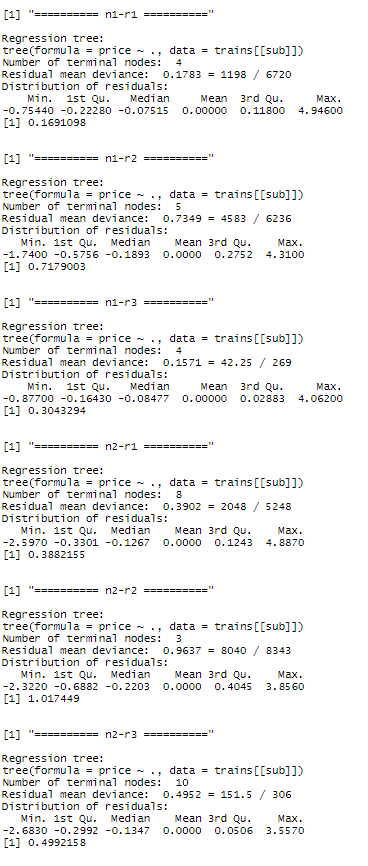
\includegraphics[width=.7\linewidth]{figures/dt2.PNG} 
   \end{minipage}\hfill
   \begin{minipage}{0.48\textwidth}
     \centering
     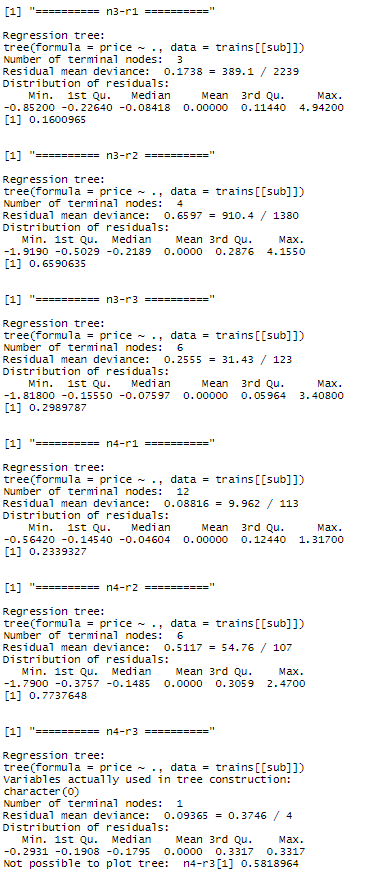
\includegraphics[width=.7\linewidth]{figures/dt3.PNG}
   \end{minipage}
   
    \begin{minipage}{0.48\textwidth}
     \centering
     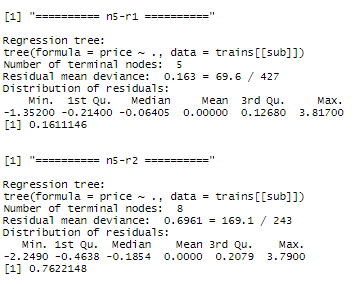
\includegraphics[width=.7\linewidth]{figures/dt4.1.PNG}
   \end{minipage}
   
   
    \begin{minipage}{0.48\textwidth}
     \centering
     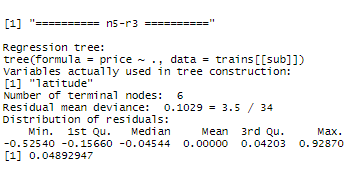
\includegraphics[width=.7\linewidth]{figures/dt4.2.PNG}
   \end{minipage}
        \caption{ Decision tree results for specific neighbourhood group and room type}\label{fig:12}

\end{figure}

\newpage
\subsubsection{Random Forest Results}
\textbf{Random Forest  on the entire dataset}\\
Random Forest on the entire dataset outputs an explained variance of $42\%$ which is acceptable and also the MSE is lower with respect to the models before. 
\begin{figure}[h]
\centering
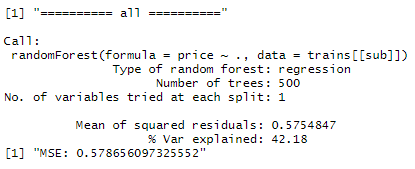
\includegraphics[width=0.7\textwidth]{figures/rf.PNG} 
 \caption{\label{fig:13} Random Forest results on the entire dataset}
\end{figure}

\noindent \textbf{Random Forest for specific neighbourhood group}\\
Random Forest on specific neighbourhood outputs overall MSE lower than the last two models. Explained variance are acceptable: for Brooklyn and Manhattan is approximately around $40\%$, $37\%$ for Queens and about $25\%$ for Staten Island and Bronx. 
\begin{figure}[!htb]
   \begin{minipage}{0.48\textwidth}
     \centering
     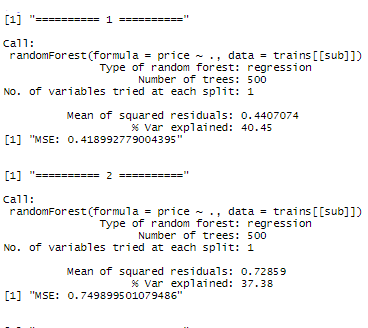
\includegraphics[width=1\linewidth]{figures/rf1.1.png} 
   \end{minipage}\hfill
   \begin{minipage}{0.48\textwidth}
     \centering
     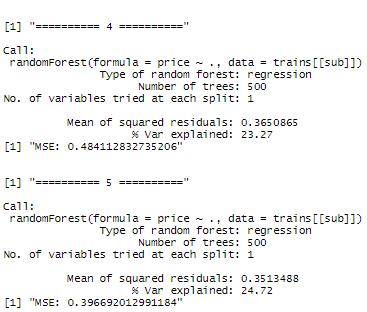
\includegraphics[width=1\linewidth]{figures/rf1.2.png}
   \end{minipage}
        \caption{ Random Forest results for specific neighbourhood group}\label{fig:14}

\end{figure}

\newpage
\noindent \textbf{Random Forest  for specific neighbourhood group and room type}\\
Random Forest for specific neighbourhood and room type does perform poorly since in some cases explained variance is negative. This could be due to the fact of overfitting, but in this case is more probable the problem is underfitting since in some specific case there is a low number of information.
\begin{figure}[!htb]
   \begin{minipage}{0.33\textwidth}
     \centering
     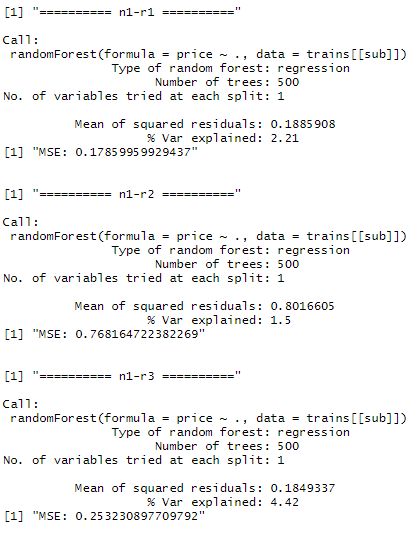
\includegraphics[width=1\linewidth]{figures/rf2.png} 
   \end{minipage}\hfill
   \begin{minipage}{0.33\textwidth}
     \centering
     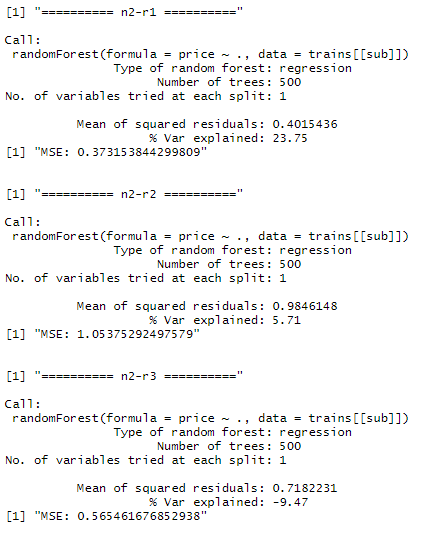
\includegraphics[width=1\linewidth]{figures/rf3.png}
   \end{minipage}
   \begin{minipage}{0.33\textwidth}
     \centering
     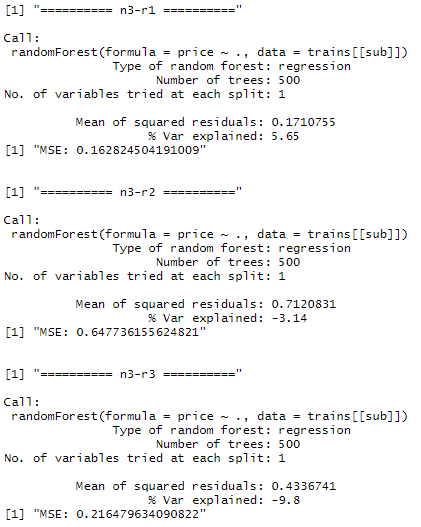
\includegraphics[width=1\linewidth]{figures/rf4.png} 
   \end{minipage}\hfill
   \begin{minipage}{0.33\textwidth}
     \centering
     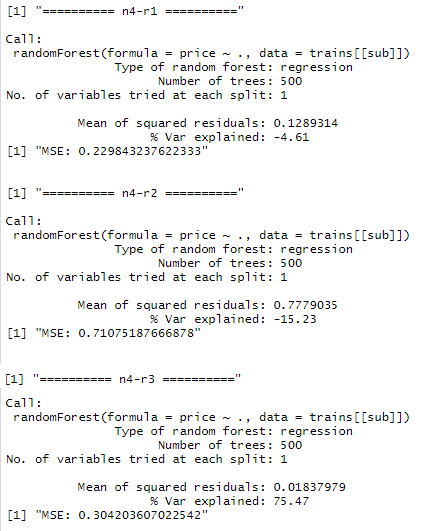
\includegraphics[width=1\linewidth]{figures/rf5.png}
   \end{minipage}
   \begin{minipage}{0.33\textwidth}
     \centering
     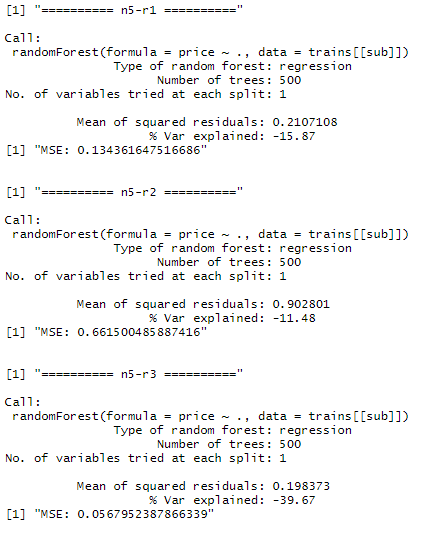
\includegraphics[width=1\linewidth]{figures/rf6.png}
   \end{minipage}
        \caption{Random Forest results for specific neighbourhood group and room type}\label{fig:15}

\end{figure}

\newpage
\subsubsection{Ranger Random Forest Results}
Ranger Random Forest is known to be computationally light with respect to the classic Random Forest. In fact, for the tuning part there were not problem in running it for the entire dataset. 
\\\\ \textbf{Ranger on the entire dataset }\\
Ranger outputs for the entire dataset are consistent. We have a $R^2$ of 0.47 and OOB error of .

\begin{figure}[h]
\centering
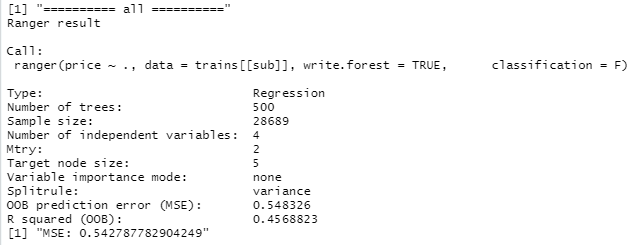
\includegraphics[width=0.7\textwidth]{figures/rgn.PNG} 
 \caption{\label{fig:16} Ranger Random Forest results on the entire dataset}
\end{figure}

\noindent \textbf{Ranger for specific neighbourhood group}\\
For the specific neighbourhood group Ranger gives different results. 
\begin{figure}[!htb]
   \begin{minipage}{0.48\textwidth}
     \centering
     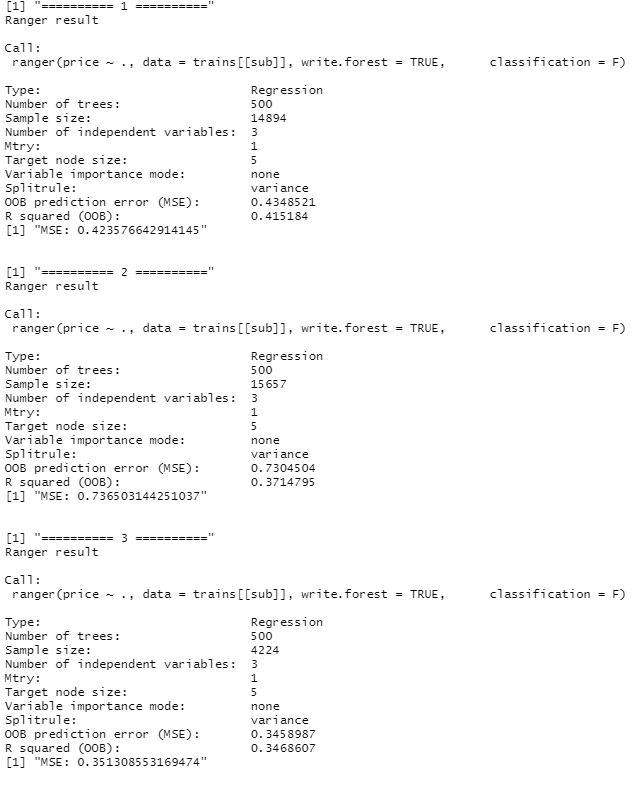
\includegraphics[width=1\linewidth]{figures/rgn1.1.png} 
   \end{minipage}\hfill
   \begin{minipage}{0.48\textwidth}
     \centering
     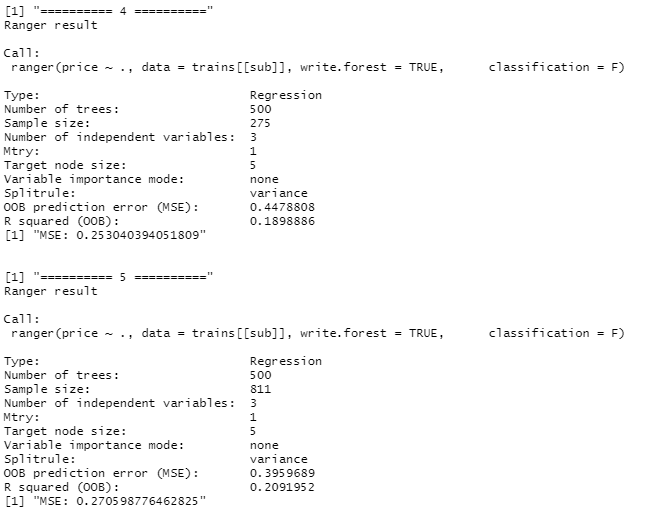
\includegraphics[width=1\linewidth]{figures/rgn1.2.png}
   \end{minipage}
        \caption{Ranger Random Forest results for specific neighbourhood group}\label{fig:17}

\end{figure}
\noindent \textbf{Ranger for specific neighbourhood group and room type}\\
The dataset filtered by neighbourhood and room type gives as result a $R^2$ of 0.25.
\begin{figure}[!htb]
   \begin{minipage}{0.48\textwidth}
     \centering
     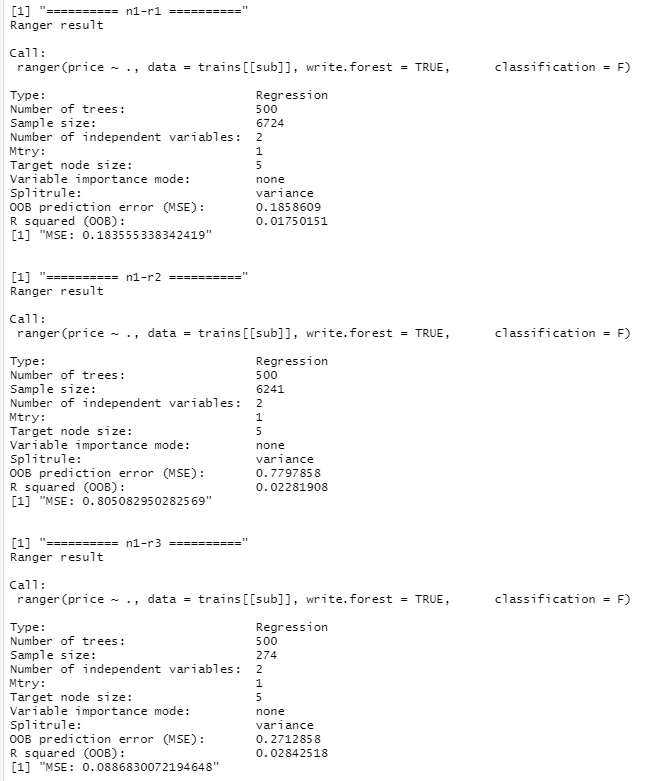
\includegraphics[width=1\linewidth]{figures/rgn2.1.png} 
   \end{minipage}\hfill
   \begin{minipage}{0.48\textwidth}
     \centering
     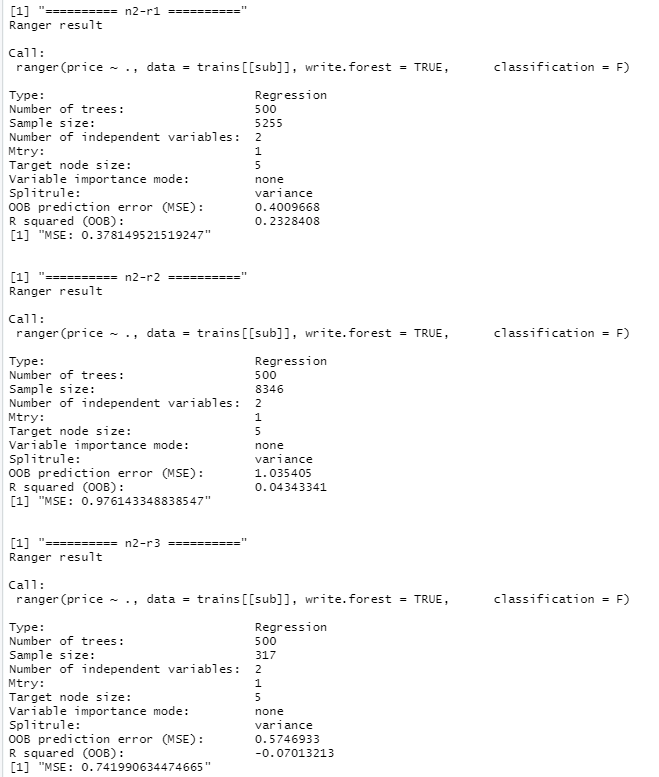
\includegraphics[width=1\linewidth]{figures/rgn2.2.png}
   \end{minipage}
   \begin{minipage}{0.48\textwidth}
     \centering
     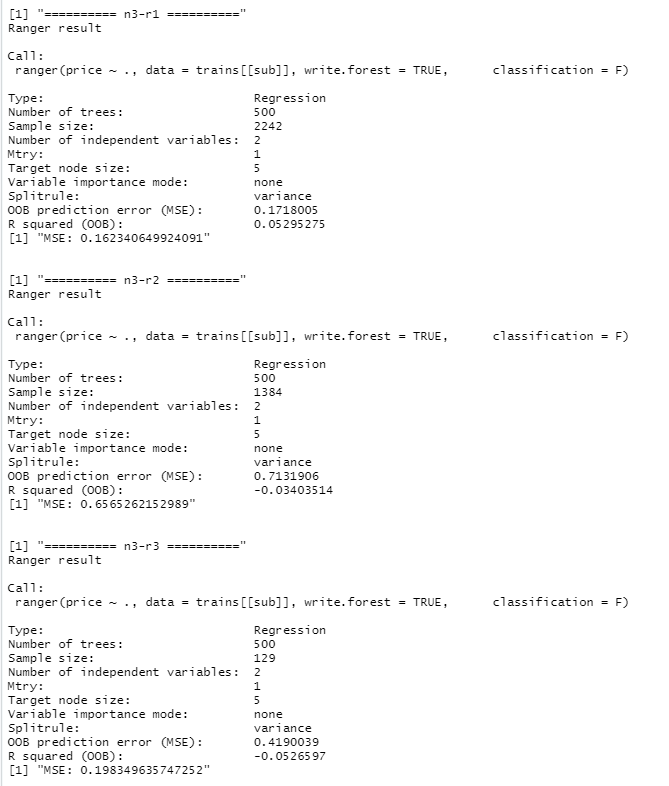
\includegraphics[width=1\linewidth]{figures/rgn2.3.png} 
   \end{minipage}\hfill
   
\end{figure}

\newpage
\begin{figure}[!htb]
   \begin{minipage}{0.48\textwidth}
     \centering
     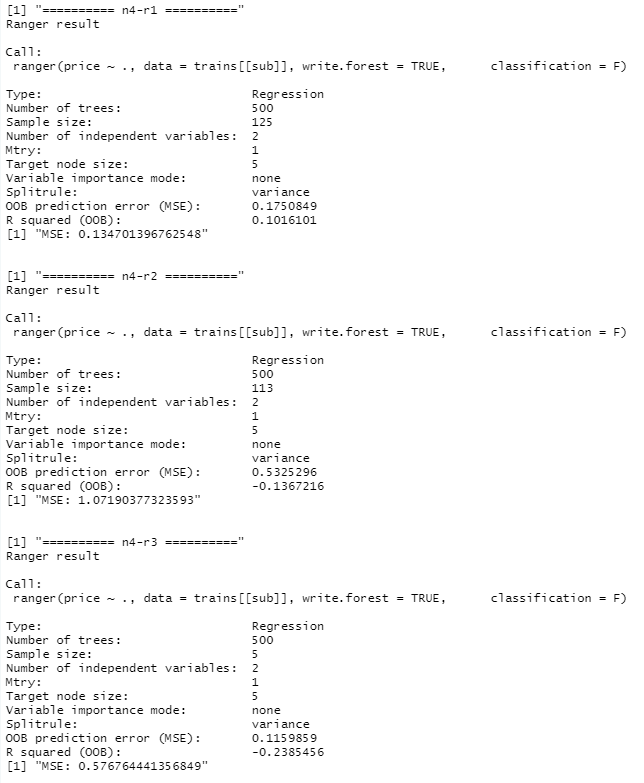
\includegraphics[width=1\linewidth]{figures/rgn2.4.png}
   \end{minipage}
   \begin{minipage}{0.48\textwidth}
     \centering
     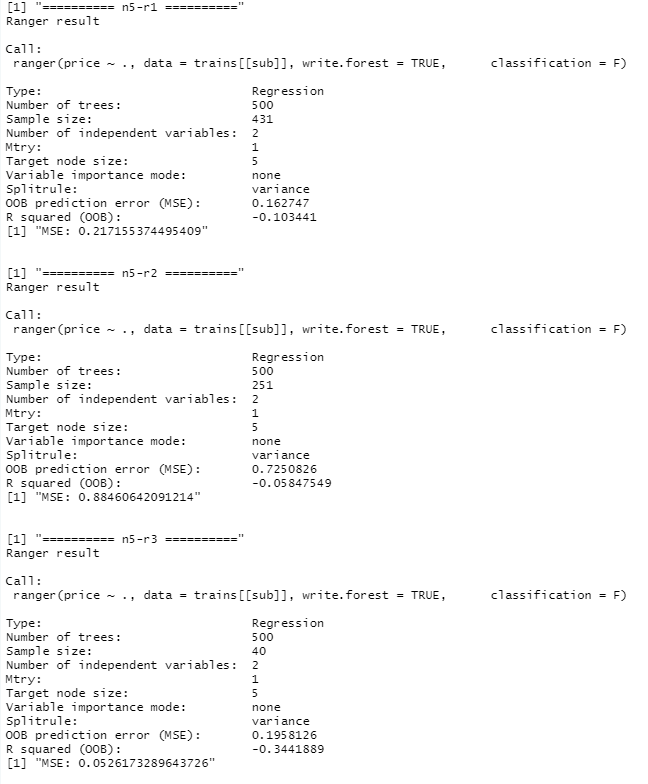
\includegraphics[width=1\linewidth]{figures/rgn2.5.png}
   \end{minipage}
        \caption{Ranger Random Forest results for specific neighbourhood group and room type}\label{fig:18}

\end{figure}





\newpage
\subsubsection{Neural Network Results}
 Neural Network on the entire dataset has been run for 30 epochs. For simplicity, it has been used a single architecture for all the subsets. It has been used three dense layers of respectively 32, 16 and 1 units and Relu activation function.\\\\
\textbf{Neural Networks on the entire dataset }\\
\noindent
For the entire dataset, the results are acceptable but not in line with random forest and the other regression methods. The model MSE and loss decrease during the epochs and it stabilise both for validation and training at the 15th epoch.
\begin{figure}[h]
\centering
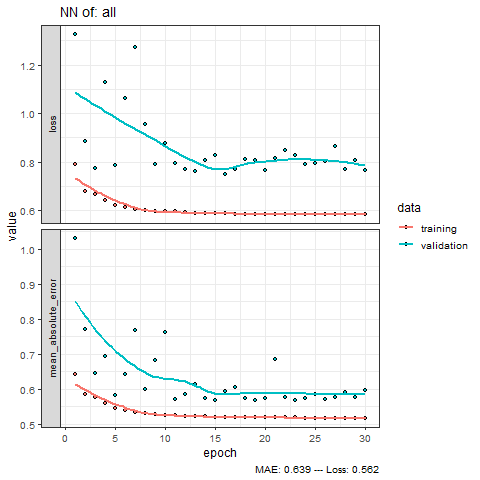
\includegraphics[width=0.7\textwidth]{figures/NN-all.PNG} 
 \caption{\label{fig:19} Neural Networks results on the entire dataset}
\end{figure}

\newpage
\noindent \textbf{Neural Networks for specific neighbourhood group}\\
For the specific group, the models output different results. The most populous such as Brooklyn and Manhattan and Queens they have a decreasing MSE and loss trend. Only for Manhattan, the validation loss seems to increase approximately after the 18th epochs. For the remaining neighbourhood they have a decreasing training and validation MSE and loss, while the validation remains stable for all the epochs.
\begin{figure}[!htb]
   \begin{minipage}{0.33\textwidth}
     \centering
     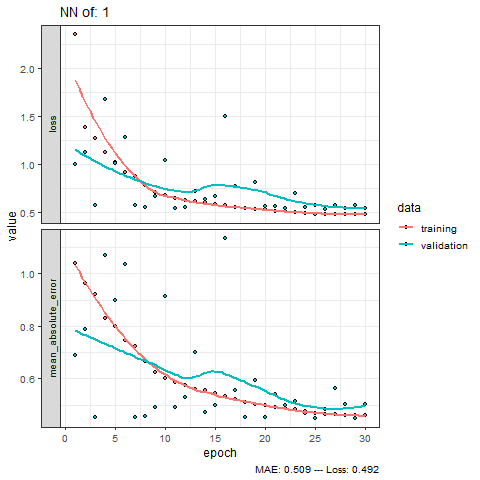
\includegraphics[width=1\linewidth]{figures/NN-1.png} 
   \end{minipage}\hfill
   \begin{minipage}{0.33\textwidth}
     \centering
     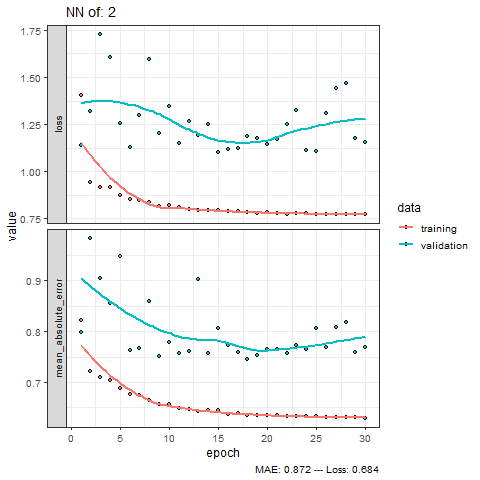
\includegraphics[width=1\linewidth]{figures/NN-2.png}
   \end{minipage}
   \begin{minipage}{0.33\textwidth}
     \centering
     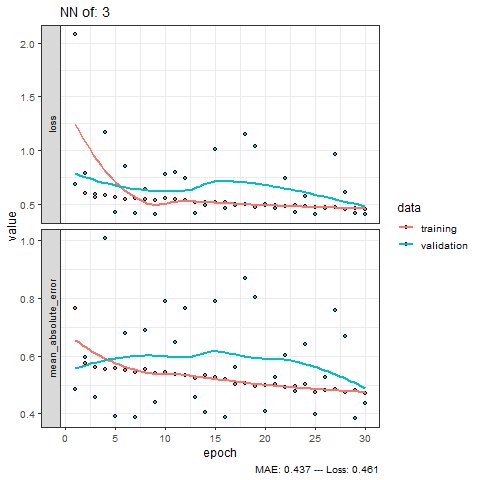
\includegraphics[width=1\linewidth]{figures/NN-3.png} 
   \end{minipage}\hfill
   \begin{minipage}{0.33\textwidth}
     \centering
     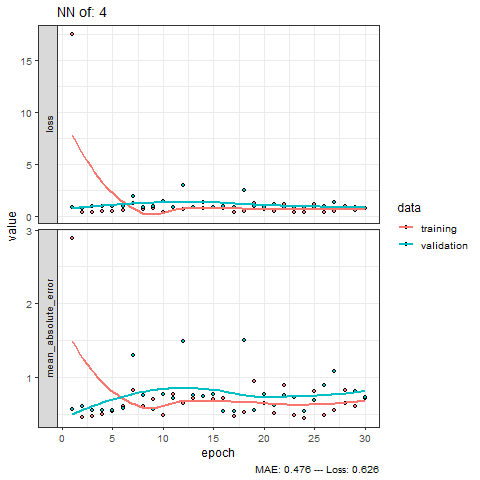
\includegraphics[width=1\linewidth]{figures/NN-4.png}
   \end{minipage}
   \begin{minipage}{0.33\textwidth}
     \centering
     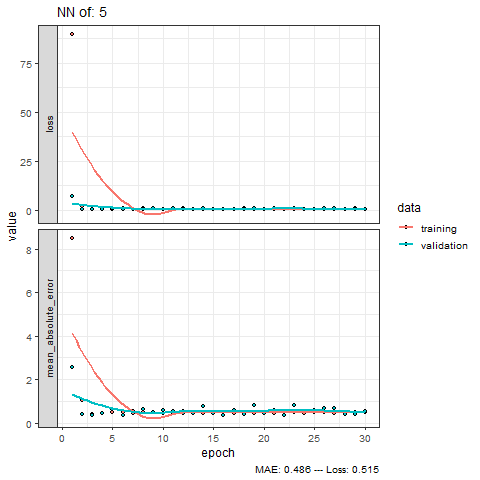
\includegraphics[width=1\linewidth]{figures/NN-5.png}
   \end{minipage}
        \caption{Neurala Networks results for specific neighbourhood group and room type}\label{fig:20}

\end{figure}

\newpage 
\noindent \textbf{Neural Networks  for specific neighbourhood group and room type}\\
For the different type of room and neighbourhood in some cases are not satisfactory while in other cases are acceptable. For the type Private room results for Brooklyn and Manhattan and Queens results in a decreasing training MSE and loss and a stable validation MSE and loss. For Brooklyn validation MSE and loss remains nearby 0, for Manhattan instead, are a bit higher compared to the training. For the last two neighbourhood starts with a very high loss and MSE train and validation, while during the epochs the value converge to a lower value near 0.5.
\\ For the entire apartment type, for Brooklyn training MSE and loss have a decreasing trend, while validation after 12th epochs increases and get value higher than the starting point. 
For Manhattan instead we have both train and validation decreasing trend, in particular slightly for the validation. For Queens validation MSE increases till epoch 18th and then decrease until it reaches almost the training MSE at the 30th epochs; while for the loss it continuously increase and decrease for all the epochs. For Bronx and State Island decreasing training MSE and loss, while a stable validation MSE.  \\ For Shared rooms similar trends of validation and train for the Brooklyn, Manhattan and Queens, starting from a high value. For State Island and Bronx results are decreases very fast but reaching high values of MAE and loss. For Staten Island, train and validation start from a loss value higher than 1000, which is very high considering the dimension of this subsets.  

\newpage
\begin{figure}[!htb]
   \begin{minipage}{0.33\textwidth}
     \centering
     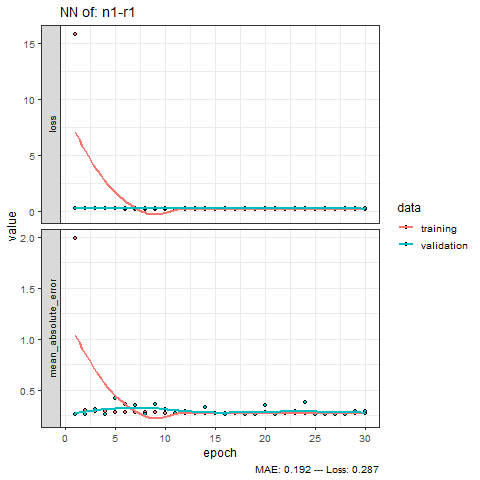
\includegraphics[width=1\linewidth]{figures/NN-n1-r1.png} 
   \end{minipage}\hfill
   \begin{minipage}{0.33\textwidth}
     \centering
     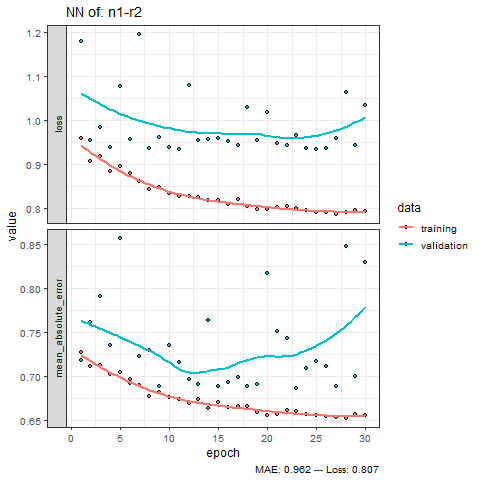
\includegraphics[width=1\linewidth]{figures/NN-n1-r2.png}
   \end{minipage}
   \begin{minipage}{0.33\textwidth}
     \centering
     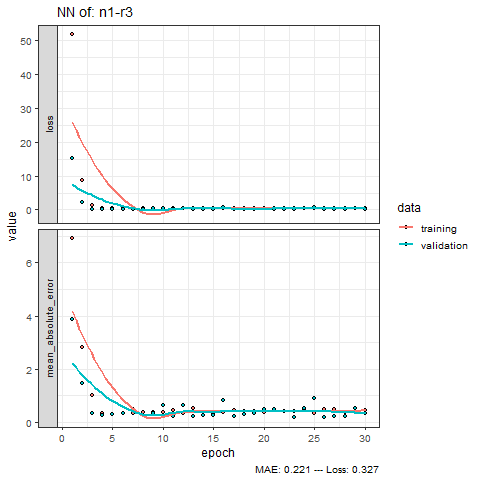
\includegraphics[width=1\linewidth]{figures/NN-n1-r3.png} 
   \end{minipage}\hfill
   \begin{minipage}{0.33\textwidth}
     \centering
     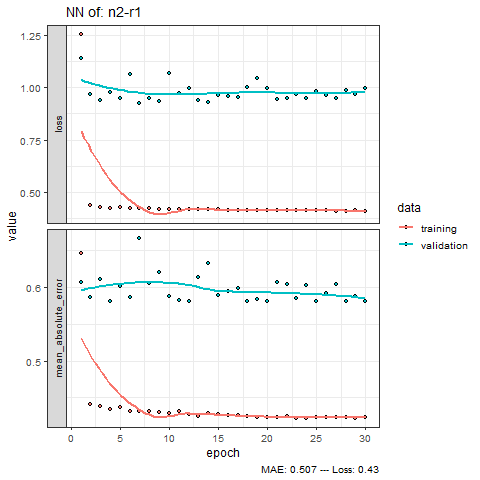
\includegraphics[width=1\linewidth]{figures/NN-n2-r1.png}
   \end{minipage}
   \begin{minipage}{0.33\textwidth}
     \centering
     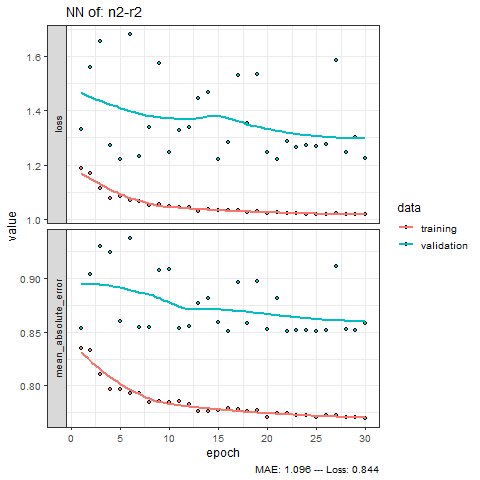
\includegraphics[width=1\linewidth]{figures/NN-n2-r2.png}
   \end{minipage}
 \begin{minipage}{0.33\textwidth}
     \centering
     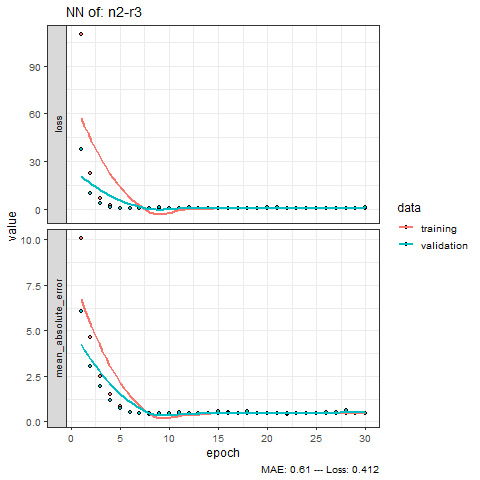
\includegraphics[width=1\linewidth]{figures/NN-n2-r3.png} 
   \end{minipage}\hfill
\begin{minipage}{0.33\textwidth}
     \centering
     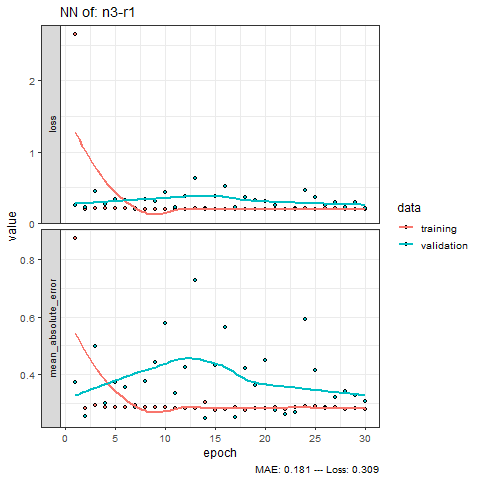
\includegraphics[width=1\linewidth]{figures/NN-n3-r1.png} 
   \end{minipage}\hfill
   \begin{minipage}{0.33\textwidth}
     \centering
     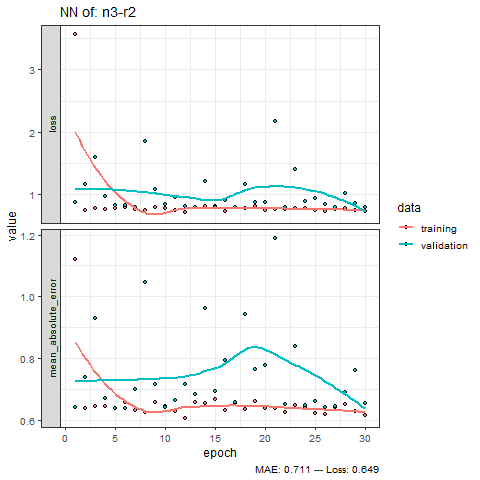
\includegraphics[width=1\linewidth]{figures/NN-n3-r2.png}
   \end{minipage}
   \begin{minipage}{0.33\textwidth}
     \centering
     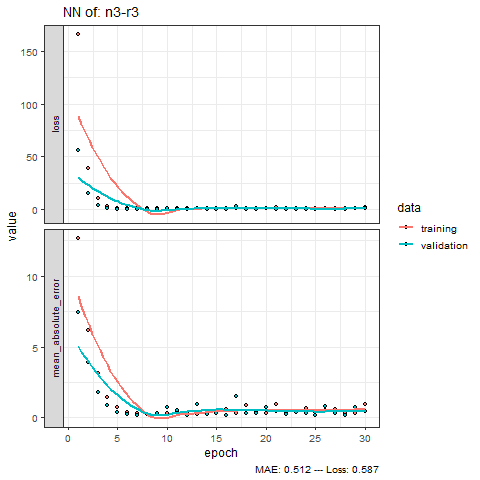
\includegraphics[width=1\linewidth]{figures/NN-n3-r3.png} 
   \end{minipage}\hfill 
\end{figure}
\begin{figure}[!htb]

   \begin{minipage}{0.33\textwidth}
     \centering
     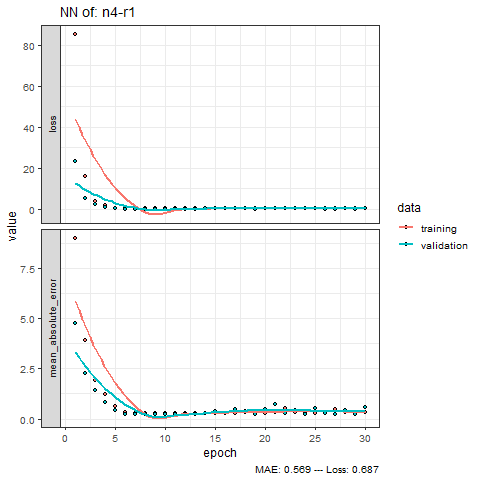
\includegraphics[width=1\linewidth]{figures/NN-n4-r1.png} 
   \end{minipage}\hfill
   \begin{minipage}{0.33\textwidth}
     \centering
     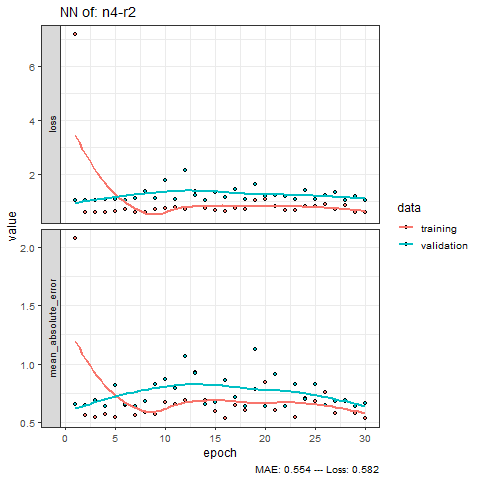
\includegraphics[width=1\linewidth]{figures/NN-n4-r2.png}
   \end{minipage}
   \begin{minipage}{0.33\textwidth}
     \centering
     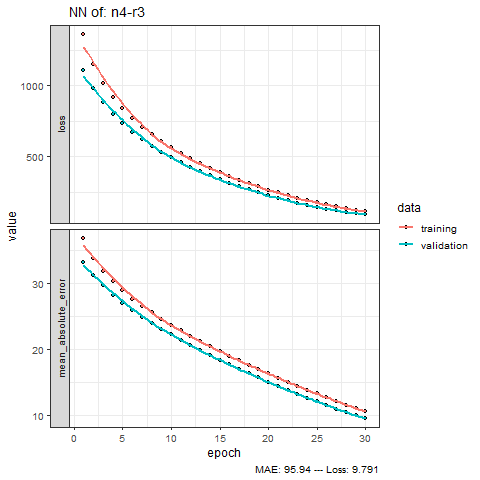
\includegraphics[width=1\linewidth]{figures/NN-n4-r3.png} 
   \end{minipage}\hfill
 

   
   \begin{minipage}{0.33\textwidth}
     \centering
     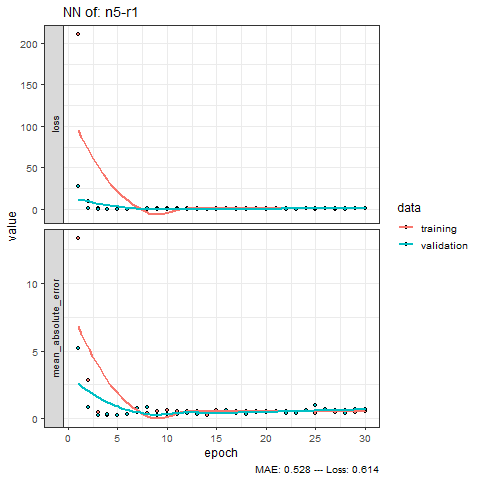
\includegraphics[width=1\linewidth]{figures/NN-n5-r1.png} 
   \end{minipage}\hfill
   \begin{minipage}{0.33\textwidth}
     \centering
     \includegraphics[width=1\linewidth]{figures/NN-n5-r2.png}
   \end{minipage}
   \begin{minipage}{0.33\textwidth}
     \centering
     \includegraphics[width=1\linewidth]{figures/NN-n5-r3.png} 
   \end{minipage}\hfill
           \caption{Neural Networks results for specific neighbourhood group and room type}\label{fig:21}

\end{figure}





\newpage
\noindent \subsubsection{K-means Results}

K-means algorithm has been run on all type of subsets as in the models before. Moreover, since the variables are not all numerical, it has been used a specific library called "clustMixType" which computes k-prototypes clustering for mixed-type data. It uses Euclidean distance for numerical variables and simple match coefficient. For simplicity has been computed only setting k = 5 since changing the value for all the different subset will be computationally and timely expensive. \\\\
As shown in the cluster map of the entire dataset, clusters define and divides the different neighbourhood. Manhattan is divided in the north and south part that also includes a part of Brooklyn. This should be the case of the most expensive houses in the entire NY city. All cluster can is a a partition of price zone in the entire city. As shown in the Figure \ref{fig:23} the distributions of prices and room type differ in the different clusters.
\begin{figure}[!htb]
   \begin{minipage}{0.48\textwidth}
     \centering
    \includegraphics[width=1\textwidth]{figures/clust-all.PNG} 
 \caption{\label{fig:22} K-means on entire dataset}
   \end{minipage}\hfill
   \begin{minipage}{0.48\textwidth}
     \centering
       \includegraphics[width=1\textwidth]{figures/clust-summary.PNG} 
 \caption{\label{fig:23} Distribution of each cluster}
   \end{minipage}
   
\end{figure}

\newpage
\noindent The maps plot clusters for the single neighbourhood (Figure \ref{fig:24}). It also shows how the data are distributed  in the maps. 
\begin{itemize}
\itemsep0em 
\item Brooklyn has 3 main visible clusters;
\item Manhattan has 2 clusters for north and south part; 
\item Queens instead has 4 visible cluster depending on the nearness to the seaside, Manhattan/Brooklyn and inland. 
\item Staten Island has spars cluster depending on the north east part or the south-west.
\item Bronx has 4 clusters visible in which 2 are mixed and the other two depends on the nearness to Manhattan.
\end{itemize}

\begin{figure}[!htb]
   \begin{minipage}{0.33\textwidth}
     \centering
     \includegraphics[width=1\linewidth]{figures/clust-1.png} 
   \end{minipage}\hfill
   \begin{minipage}{0.33\textwidth}
     \centering
     \includegraphics[width=1\linewidth]{figures/clust-2.png}
   \end{minipage}
   \begin{minipage}{0.33\textwidth}
     \centering
     \includegraphics[width=1\linewidth]{figures/clust-3.png} 
   \end{minipage}\hfill
   \begin{minipage}{0.33\textwidth}
     \centering
     \includegraphics[width=1\linewidth]{figures/clust-4.png}
   \end{minipage}
   \begin{minipage}{0.33\textwidth}
     \centering
     \includegraphics[width=1\linewidth]{figures/clust-5.png}
   \end{minipage}
        \caption{K-means for specific neighbourhood group}\label{fig:24}
\end{figure}
\newpage
\noindent 
Clusters for specific neighbourhood group and room type have a similar shape changing the room type. 
\begin{itemize}
\itemsep0em 
\item Brooklyn: 
\begin{itemize}
\itemsep0em 
\item Private room 4 visible clusters distinguishable from the others based on the position.
\item Entire Apartment 4 visible cluster but less distinguishable with respect to the private rooms. One cluster has a distribution of small number of points for all the neighbourhood.
\item Shared room 4 visible cluster but the south is not dominated by only one cluster but now is split in two parts. To be notice that there are a smaller number of shared rooms on the east part.
\end{itemize} main visible clusters;
\item Manhattan :
\begin{itemize}
\itemsep0em 
\item Private room is divided in three main clusters based on the position. This could be due to the fact that prices change in between downtown, midtown and uptown.
\item Entire apartment has similar shape as the private room, but the uptown cluster is smaller.
\item Shared room similar shape but are less distributed in the downtown part. 
\end{itemize}

\item Queens:
\begin{itemize}
\itemsep0em 
\item Private room has a distinc shape of the 5 clusters based on the zones. 
\item Entire apartment room instead, has a mix shape of cluster in the zone nearby Brooklyn/Manhattan and near the airport zone (south east) 
\item Shared room are not so much and more distributed in the inland and nearby Brooklyn/Manhattan 
\end{itemize}


\begin{figure}[!htb]
   \begin{minipage}{0.33\textwidth}
     \centering
     \includegraphics[width=1\linewidth]{figures/clust-n1-r1.png} 
   \end{minipage}\hfill
   \begin{minipage}{0.33\textwidth}
     \centering
     \includegraphics[width=1\linewidth]{figures/clust-n1-r2.png}
   \end{minipage}
   \begin{minipage}{0.33\textwidth}
     \centering
     \includegraphics[width=1\linewidth]{figures/clust-n1-r3.png} 
   \end{minipage}\hfill
   \begin{minipage}{0.33\textwidth}
     \centering
     \includegraphics[width=1\linewidth]{figures/clust-n2-r1.png}
   \end{minipage}
   \begin{minipage}{0.33\textwidth}
     \centering
     \includegraphics[width=1\linewidth]{figures/clust-n2-r2.png}
   \end{minipage}
 \begin{minipage}{0.33\textwidth}
     \centering
     \includegraphics[width=1\linewidth]{figures/clust-n2-r3.png} 
   \end{minipage}\hfill
\begin{minipage}{0.33\textwidth}
     \centering
     \includegraphics[width=1\linewidth]{figures/clust-n3-r1.png} 
   \end{minipage}\hfill
   \begin{minipage}{0.33\textwidth}
     \centering
     \includegraphics[width=1\linewidth]{figures/clust-n3-r2.png}
   \end{minipage}
   \begin{minipage}{0.33\textwidth}
     \centering
     \includegraphics[width=1\linewidth]{figures/clust-n3-r3.png} 
   \end{minipage}\hfill 
\end{figure}

\newpage

\item Staten Island:
\begin{itemize}
\itemsep0em 
\item Private room are visible 4 clusters that are based on the position.
\item Entire apartment 3 greater and visible clusters, one near the border of New Jersey and Queens, one on the east coast and one more in the inland. 
\item Shared room are very small number, and clustering is not very useful in this case since it is not possible to see more than 2 clusters from 4 points. Which is not very informative.
\end{itemize}
\item Bronx:
\begin{itemize}
\itemsep0em 
\item Private room are visible 4 clusters depending on the nearness to Manhattan and the position since the prices will change based on the neighbour.
\item Entire apartment  4 clusters visible and a shape similar to the private room but with less points.
\item Shared Room 4 clusters visible but low number of points. 

\end{itemize}


\begin{figure}[!htb]
   \begin{minipage}{0.33\textwidth}
     \centering
     \includegraphics[width=1\linewidth]{figures/clust-n4-r1.png} 
   \end{minipage}\hfill
   \begin{minipage}{0.33\textwidth}
     \centering
     \includegraphics[width=1\linewidth]{figures/clust-n4-r2.png}
   \end{minipage}
   \begin{minipage}{0.33\textwidth}
     \centering
     \includegraphics[width=1\linewidth]{figures/clust-n4-r3.png} 
   \end{minipage}\hfill
 

   
   \begin{minipage}{0.33\textwidth}
     \centering
     \includegraphics[width=1\linewidth]{figures/clust-n5-r1.png} 
   \end{minipage}\hfill
   \begin{minipage}{0.33\textwidth}
     \centering
     \includegraphics[width=1\linewidth]{figures/clust-n5-r2.png}
   \end{minipage}
   \begin{minipage}{0.33\textwidth}
     \centering
     \includegraphics[width=1\linewidth]{figures/clust-n5-r3.png} 
   \end{minipage}\hfill
           \caption{K-means for specific neighbourhood group and room type}\label{fig:25}

\end{figure}
\end{itemize}

\newpage



\newpage
\noindent \textbf{Hierarchical Cluster Analysis}\\
For this type of method dataset is different with respect to those of the other methods. The reason is that obtaining a dendrogram  for all the possible houses is not informative, since the output of the Hierarchical Cluster will be a dendrogram  in which each label is the correspondent id of the column. For this reason, the dataset has been aggregate using the mean of the prices depending on the case. To compute the distances has been used the Gower distances and complete linkage method for HC.
\\\\
\noindent  As shown in Figure \ref{fig:26} the dendrogram  is generated from the dataset that has been aggregate for mean of the neighbourhood and also for the type of room obtaining the mean of the prices for each case. From Figure \ref{fig:27} is possible to see how giving a certain interval of 0.6 the coloured branches are those that could be consider in the same cluster for the HC algorithm. 
\begin{figure}[!htb]
   \begin{minipage}{0.48\textwidth}
     \centering
    \includegraphics[width=1\textwidth]{figures/hc.PNG} 
 \caption{\label{fig:26} Hierarchical Clustering}
   \end{minipage}\hfill
   \begin{minipage}{0.48\textwidth}
     \centering
       \includegraphics[width=1\textwidth]{figures/hc2.PNG} 
 \caption{\label{fig:27} Hierarchical Clustering coloured }
   \end{minipage}
   
\end{figure}
\\
\noindent From Figure \ref{fig:27} is possible to see the dendrogram  for the case of the mean for each neighbourhood without considering the single case for the room type. 



\begin{figure}[h]
  \centering
    \includegraphics[width=0.7\textwidth]{figures/hc3.PNG} 
 \caption{\label{fig:28} Hierarchical Clustering}
\end{figure}

\newpage
\noindent \subsubsection{Principal Component Analysis Results}

\textbf{PCA mixed type}\\
PCA on mixed type of data has been applied on the entire dataset, since the neighbourhood subsets are small and there is no need to apply a dimensionality reduction. The resulting subset have only two dimensions filtering for room type and neighbourhood. Without filters the dimension became four, not so much also in this case but could be interesting to know if the data could be reduced more without losing too much information. 
\\\\
From Figure \ref{fig:29} is possible to see the Eigenvalues for each dimension and the proportion of each one to the proportion and cumulative values of variance explained. Three and four dimensions correspond respectively to a cumulative variance explained of $68\%$ and $79\%$ which could be acceptable to get almost the explained variance of all the nine dimensions but with less dimensions. 
\\
Figure \ref{fig:30} shows how qualitative and quantitative variables are correlated with the different dimensions.
\begin{figure}[!htb]
   \begin{minipage}{0.48\textwidth}
     \centering
    \includegraphics[width=1\textwidth]{figures/pcamix.PNG} 
 \caption{\label{fig:29} PCA on mixed type of data}
   \end{minipage}\hfill
   \begin{minipage}{0.48\textwidth}
     \centering
       \includegraphics[width=1\textwidth]{figures/pcamix2.PNG} 
 \caption{\label{fig:30} Varible correlation with each dimension }
   \end{minipage}
   
\end{figure}

\noindent 
\\\\
\textbf{Factor Analysis of Mixed Data (FAMD)}\\
Factor analysis is a technique that is used to reduce a large number of variables into fewer numbers of factors. 
\\
It has been applied on the entire dataset also in this case. From Figure \ref{fig:Figure 31} it is possible to see how explained variance of each dimension is changing. The results are the same of the PCA mixed type library. 
\\\\
\noindent Figure \ref{fig:32} is the scree plot that displays how much variation each principal component captures from the data.

\begin{figure}[!htb]
   \begin{minipage}{0.48\textwidth}
     \centering
    \includegraphics[width=1\textwidth]{figures/FAMD.PNG} 
 \caption{\label{fig:31} Eigenvalues and explained variance results}
   \end{minipage}\hfill
   \begin{minipage}{0.48\textwidth}
     \centering
       \includegraphics[width=1\textwidth]{figures/FAMD2.PNG} 
 \caption{\label{fig:32} Scree plot }
   \end{minipage}
   
\end{figure}
\noindent Figure \ref{fig:33} shows the relationship between variables, the quality of the representation of variables, as well as, the correlation between quantitative variables and the dimensions.
\begin{itemize}
\itemsep0em 
\item price has a negative correlation with the first dimension and almost no correlation to the second one. Price also has a low  quality of representation on the factor map. 
\item latitude has a strong correlation to the second dimensions and almost no correlation to the first one. Latitude has an high quality of representation. 
\item longitude has a strong correlation on the first dimension and a modest on the second one. Longitude has a medium quality of representation.
\end{itemize}
Figure \ref{fig:34}  shows the qualitative variable contribution to each dimension:
\begin{itemize}
\item neighborhood group with high number of houses has the highest quality of representation, while Bronx and Staten Island has low contribution.
\item room types have low contribution with respect to the neighbourhood but Entire home and Private room has more than Shared room that in the plot appears to be the worst variable in term of contribution. 
\end{itemize}



\begin{figure}[!htb]
   \begin{minipage}{0.48\textwidth}
     \centering
    \includegraphics[width=1\textwidth]{figures/FAMD3.PNG} 
 \caption{\label{fig:33} Quantitative variable contribution}
   \end{minipage}\hfill
   \begin{minipage}{0.48\textwidth}
     \centering
       \includegraphics[width=1\textwidth]{figures/FAMD4.PNG} 
 \caption{\label{fig:34} Qualitative variable contribution }
   \end{minipage}
   
\end{figure}

\noindent Figure \ref{fig:35} shows in the first group the coordinates of the variable; the second group represent the Cos2, which is the quality of representation on the factor map; the third values are the contribution of each variables to the dimensions. 
\\\\
Figure \ref{fig:36} displays the summary of the correlation of all the variables to the principal dimensions.
Latitude appears to be the one most correlated with the second dimension, while longitude and price to the first one. Neighbourhood groups appears to be the most correlated with dimension one and two. Room type is modestly correlated with dimension one and not correlated to dimension two. 
\begin{figure}[!htb]
   \begin{minipage}{0.48\textwidth}
     \centering
    \includegraphics[width=1\textwidth]{figures/FAMD5.PNG} 
 \caption{\label{fig:35} Coordinates,quality of representation and contribution for each variable }
   \end{minipage}\hfill
   \begin{minipage}{0.48\textwidth}
     \centering
       \includegraphics[width=1\textwidth]{figures/FAMD6.PNG} 
 \caption{\label{fig:36} Summary of the correlation of all the variables to the first two dimensions }
   \end{minipage}
   
\end{figure}


\newpage
\noindent Figure \ref{fig:37} represents how the contribution of the variables effect each five dimension selected with an expected average value of $20\%$. It is possible to notice that the contributions are not uniform. Latitude does not contribute to the first dimension while price and room type for the second one. Longitude, latitude and price almost do not contribute to the fourth and fifth dimensions, this means that only qualitative variables effect these two dimensions.
\begin{figure}[!htb]
   \begin{minipage}{0.33\textwidth}
     \centering
     \includegraphics[width=1\linewidth]{figures/FAMD7.png} 
   \end{minipage}\hfill
   \begin{minipage}{0.33\textwidth}
     \centering
     \includegraphics[width=1\linewidth]{figures/FAMD8.png}
   \end{minipage}
   \begin{minipage}{0.33\textwidth}
     \centering
     \includegraphics[width=1\linewidth]{figures/FAMD9.png} 
   \end{minipage}\hfill
   \begin{minipage}{0.33\textwidth}
     \centering
     \includegraphics[width=1\linewidth]{figures/FAMD10.png}
   \end{minipage}
   \begin{minipage}{0.33\textwidth}
     \centering
     \includegraphics[width=1\linewidth]{figures/FAMD11.png}
   \end{minipage}
  \caption{\label{fig:37}  Contribution of all the variables to each dimension}

\end{figure}

\newpage



\section{Conclusion}
 
 
\subsection{Price prediction}
\begin{figure}[H]
\centering
\includegraphics[width=1\textwidth]{figures/model_summary.PNG} 
\caption{\label{fig:37} Summary of the MSE for all the models for each subset of the dataset }
\end{figure}
\newpage
\noindent Figure \ref{fig:37} is possible to see all the Mean Square Error for each model and case. \\
For the entire dataset, the best performance come from the Ranger Random Forest with the lowest value. Neural Network are the worst, this could be due to the fact that has not been done any  hyper parametrisation tuning since a single fixed architecture has been used. 
\\
For the specific neighbourhood groups Ranger Random Forest and Random Forest has similar predictive performance and they better with respect to the others. Only for Staten Island the Linear regression has better performance but similar to the two Random Forest.
\\ 
For the specific neighbourhood groups and room type model perform differently. It depends on the subset prediction is based so is not possible to determine the best choice. According to all the results Random Forest could maybe be the most suitable in general but it is computationally the more expensive one, so Ranger should be the better substitute. 
\\\\
For future tests, tuning of the Neural Networks (in general for all the model) could increase the price prediction precision but taking in account also the computational and time cost.
\\\\


\subsection{Clusters and groups}
The second objective has been accomplished.\\\\ Cluster definitions appeared to be consistent, price and position determined the main characteristics of the different group and it is possible to give a meaning to this division. Only for some specific subset such as Staten Island and Bronx Shared room are pour, but this is due to the fact that those subsets contains low information.
Hierarchical Cluster Analysis give also consistent results based on the price mean for each neighbourhood group and room type. This solution is an approximation, since giving the base dataset with 48000 gives result to a very confusing dendrogram  with a branch for each row which is not informative.
\\\\
Principal component analysis gives a lot of information about the variables and their contribution on the quality of the information and the correlation with the different components.



\newpage
\section{Appendix}
%\subfile{project}
The File "project-code.Rmd" is attached and contains the code.

%\includepdf[pages=-, pagecommand=\thispagestyle{plain}]{project.tex}
%\noinden



\end{document}